% !TEX root = main.tex
\section{Conclusioni: cosa aggiunge l'apprendimento}
\label{sec:conclusioni-finale}
In questa parte andiamo a esporre i vari esperimenti fatti, mostrando i risultati ottenuti da questo modello. 

\subsection{Esperimento 1: Come influisce il parametro \texorpdfstring{$\sigma_{\mathrm{target}}$}{sigma target}} 
Congelando la parte appresa ($m_\theta=1$, Moreira--Muir pura) il profilo di
rischio non cambia. Sul periodo 2015/26 il modello appreso e la formula pura hanno
lo stesso massimo drawdown entro il rumore (MDD $0.185$ vs $0.219$) e un
Calmar confrontabile ($1.24$ vs $1.13$); la rete converge sistematicamente su
$m_\theta\approx 1$ riproducendo in sostanza la regola deterministica. 

Confrontando varie versioni del modello che differiscono per il parametro $\sigma_{\mathrm{target}}$, cioè la volatilità annuale del portafoglio che
il modello cerca di mantenere, capiamo che cambiare questa variabile non porta a dei miglioramenti. 
$\sigma_{\mathrm{target}}$ è la manopola che abbiamo sul drawdown, aumentando il suo valore aumenta anche il massimo drawdown ottenuto in modo monotono, 
insomma è il parametro che ci permette di scegliere il rischio di perdita che vogliamo avere e non porta a nessun tipo di ottimizzazione dell'apprendimento.

\begin{table}[H]
\centering
\small
\caption{Esperimento 1 --- overlay appreso ($m_\theta$) vs formula
pura ($m_\theta{=}1$, Moreira--Muir) ai vari $\sigma_{\mathrm{target}}$, periodo
2015--2026 (mediana su 3 seed).}
\label{tab:exp1-mm-sweep}
\begin{tabular}{llcccc}
\toprule
$\sigma_{\mathrm{target}}$ & Overlay & cash & MDD & Calmar & Sharpe \\
\midrule
\multirow{2}{*}{0.10}
 & appreso ($m_\theta$)     & 0.790 & 0.056 & 0.85 & 1.115 \\
 & formula ($m_\theta{=}1$) & 0.615 & 0.089 & 1.04 & 1.240 \\
\midrule
\multirow{2}{*}{0.15}
 & appreso ($m_\theta$)     & 0.438 & 0.105 & 1.35 & 1.361 \\
 & formula ($m_\theta{=}1$) & 0.337 & 0.138 & 1.35 & 1.442 \\
\midrule
\multirow{2}{*}{0.20}
 & appreso ($m_\theta$)     & 0.217 & 0.185 & 1.24 & 1.466 \\
 & formula ($m_\theta{=}1$) & 0.179 & 0.219 & 1.13 & 1.471 \\
\bottomrule
\end{tabular}
\end{table}


\paragraph{Conservatività, non intelligenza.} 
Per capire se la rete neurale abbia davvero sviluppato una capacità di prevedere quando uscire dal mercato prima dei crolli, è necessario separare l'effetto del tempismo da quello del livello medio di liquidità mantenuto. 
Per farlo abbiamo tracciato una frontiera di controllo. Abbiamo preso un piano cartesiano dove l'asse x contiene il livello di cash medio mantenuto mentre l'asse y contiene l'MDD. 
Su questo piano cartesiano viene tracciata una curva che unisce le varie collocazioni della formula di volatility targeting di Moreira e Muir al variare di $\sigma_{\mathrm{target}}$. Se l'agente avesse appreso un'intelligenza predittiva superiore, dovrebbe posizionarsi al di sotto di questa curva: a parità di liquidità media, dovrebbe cioè subire perdite massime inferiori grazie alla tempestività dei suoi interventi.
(Fig.~\ref{fig:frontier}). 

I dati mostrano invece l'esatto contrario: \textbf{il modello appreso cade esattamente sulla frontiera della formula deterministica} in tutti i cinque regimi di mercato considerati. 
Gli scarti di MDD sono trascurabili e privi di un pattern sistematico. 
Questo dimostra che il drawdown minore ottenuto dal modello rispetto alla formula standard allo stesso $\sigma_{\mathrm{target}}$ non deriva da una gestione dinamica intelligente, ma semplicemente dal fatto che l'agente sceglie di rimanere mediamente più disinvestito. 
Si tratta di pura conservatività: lo stesso identico livello di protezione si può ottenere con la formula statica, limitandosi ad abbassare il bersaglio di volatilità.



\begin{figure}[H]
\centering
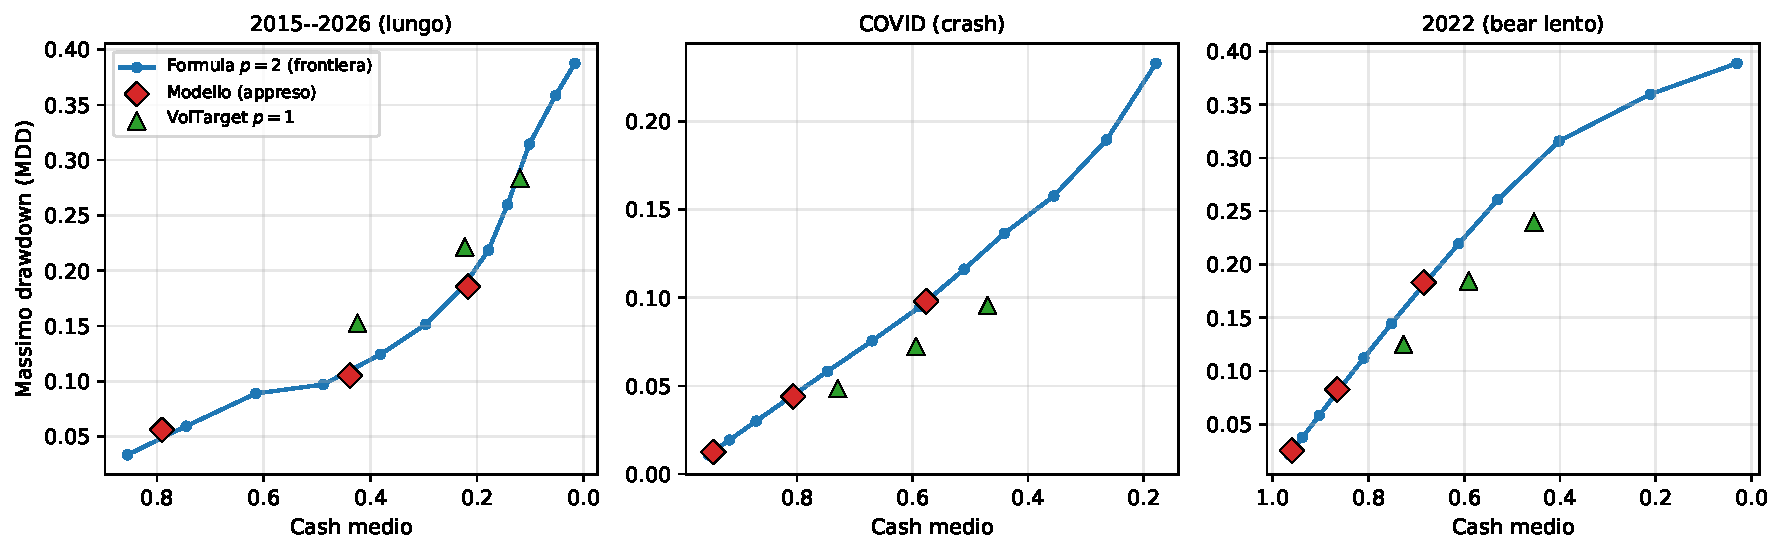
\includegraphics[width=\textwidth]{frontier_mdd.pdf}
\caption{Frontiera cash medio--MDD. Curva blu: formula fissa ($p=2$, $m_\theta=1$) al variare di $\sigma_{\mathrm{target}}$; rombi rossi: modello appreso ($\sigma_{\mathrm{target}}=0.10,\,0.15,\,0.20$); triangoli verdi: volatility targeting classico ($p=1$), stessi $\sigma_{\mathrm{target}}$.}
\label{fig:frontier}
\end{figure}



\begin{table}[H]
\centering
\caption{Confronto a $\sigma_{\mathrm{target}}=0.20$ delle quattro strategie
(mediana su 3 seed). ``modello'' $=m_\theta$ appreso; ``formula'' $=$ Moreira--Muir
pura ($p=2$); ``voltarget'' $=$ volatility targeting classico ($p=1$);
``equipesato'' $=$ paniere equipesato pienamente investito.}
\label{tab:exp1-strategie}
\begin{tabular}{llccc}
\toprule
Periodo & Strategia & MDD & Calmar & Sharpe \\
\midrule
\multirow{4}{*}{2015--26}
 & modello    & $0.185$ & $1.24$  & $1.47$ \\
 & formula    & $0.219$ & $1.13$  & $1.47$ \\
 & voltarget  & $0.284$ & $0.96$  & $1.44$ \\
 & equipesato & $0.379$ & $0.80$  & $1.25$ \\
\midrule
\multirow{4}{*}{COVID}
 & modello    & $0.098$ & $4.17$  & $2.47$ \\
 & formula    & $0.116$ & $4.05$  & $2.47$ \\
 & voltarget  & $0.096$ & $7.20$  & $2.83$ \\
 & equipesato & $0.323$ & $2.99$  & $1.71$ \\
\midrule
\multirow{4}{*}{2022}
 & modello    & $0.183$ & $-0.95$ & $-1.62$ \\
 & formula    & $0.219$ & $-0.95$ & $-1.60$ \\
 & voltarget  & $0.240$ & $-0.91$ & $-1.13$ \\
 & equipesato & $0.379$ & $-0.95$ & $-1.15$ \\
\midrule
\multirow{4}{*}{2025}
 & modello    & $0.153$ & $0.94$  & $0.98$ \\
 & formula    & $0.165$ & $0.92$  & $0.98$ \\
 & voltarget  & $0.100$ & $3.54$  & $1.95$ \\
 & equipesato & $0.227$ & $1.13$  & $1.08$ \\
\bottomrule
\end{tabular}
\end{table}

\begin{figure}[H]
\centering
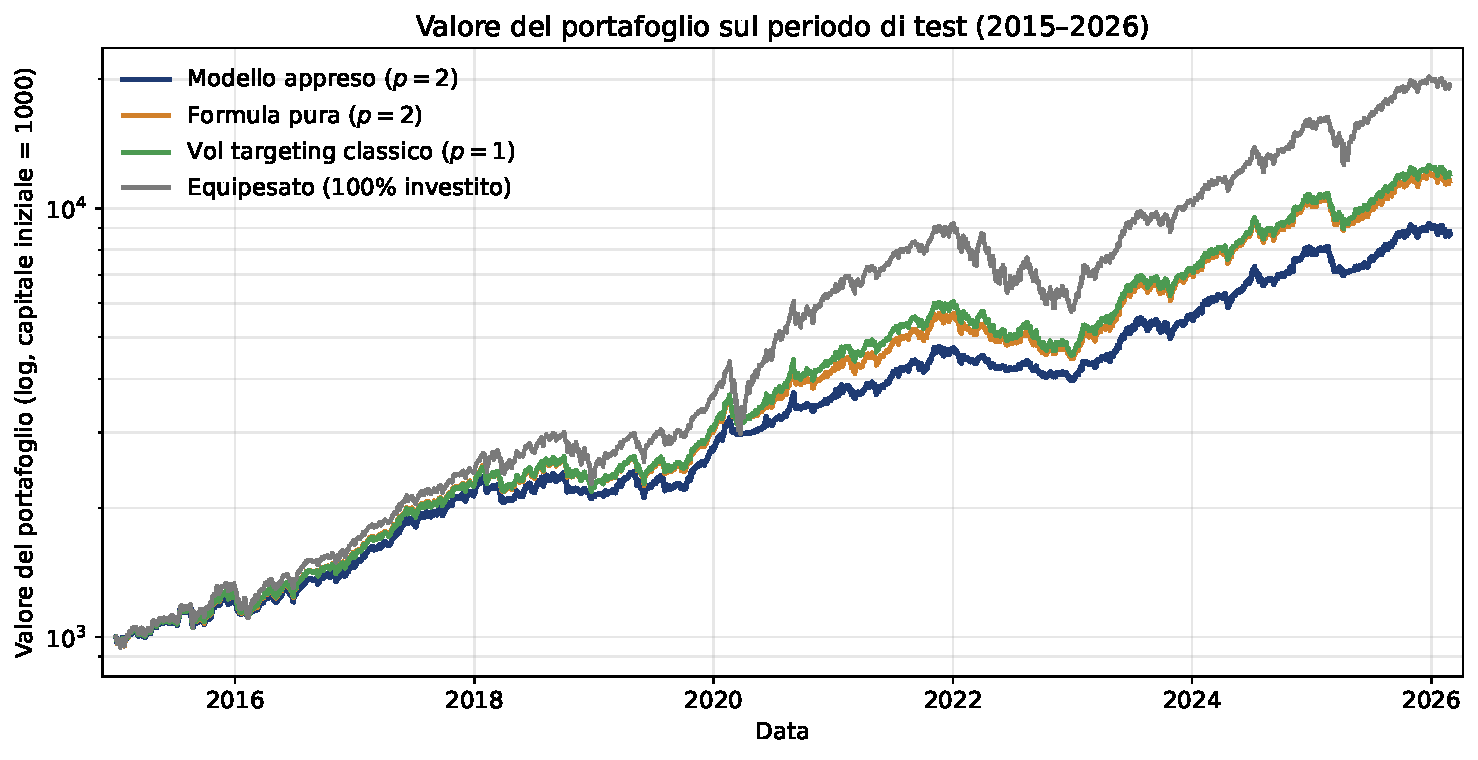
\includegraphics[width=\textwidth]{equity_curve.pdf}
\caption{Valore del portafoglio nel tempo sul periodo di test (2015--2026): modello appreso, formula pura ($p=2$), volatility targeting classico ($p=1$) ed equipesato pienamente investito.}
\label{fig:equity-curve}
\end{figure}


\subsection{Esperimento 2: L'esponente al centro delle osservazioni}

Dai risultati dello scorso esperimento abbiamo visto che il valore dell'esponente può fare la differenza in alcuni momenti del mercato grazie alla velocità e grandezza della reazione ai periodi di turbolenza, questa osservazione ci porta direttamente all'esperimento numero due.
Quando l'esponente della formula è mantenuto fisso, il valore di $p$ funge da principale leva difensiva, ma la sua efficacia dipende fortemente dal tipo di mercato:
\begin{itemize}
\item Nei crolli improvvisi e violenti (come il crash COVID del 2020 o il sell-off dei dazi del 2025) l'esponente $p=1$ si comporta meglio. 
Questo perché riducendo l'esposizione in modo più moderato evita un'uscita eccessiva che farebbe perdere il rimbalzo successivo. 
Il vantaggio è evidente soprattutto sul rendimento corretto per il rischio (Sharpe e Calmar più alti), in quanto la strategia restando parzialmente investita partecipa alla ripresa del mercato.
\item Nei ribassi lenti e prolungati (come il bear market del 2022) e sull'orizzonte storico di lungo periodo, un esponente $p=2$ contiene meglio il drawdown. 
Quando la volatilità sale, anche in modo moderato ma persistente, la reazione amplificata dal quadrato riduce la quota investita in maniera più decisa, mantenendo più liquidità.
\end{itemize}
Nessun valore fisso, dunque, riesce a dominare su tutti i contesti di mercato.


Da questa constatazione abbiamo sviluppato due esperimenti paralleli:
\begin{itemize}
    \item Rendere l'esponente $p$ apprendibile dalla rete.
    \item Imporre una regola fissa che scambia il modello dalla versione con $p=1$ a quella con $p=2$ quando vengono superati determinati limiti.
\end{itemize}

\subsubsection{Esponente appreso}
Partendo dall'ipotesi che lasciar apprendere l'esponente alla rete neurale possa permettergli di adattarsi dinamicamente al contesto si è sviluppato il seguente esperimento.

Prima di tutto la rete è stata modificata aggiungendo una nuova \lstinline{exposure_head} che si concentra sul calcolare l'esponente.
Questa testa lavora in parallelo con quella progettata per l'esposizione.
Per prendere la decisione utilizza gli stessi dati dell'altra che decide l'esposizione e ottimizza la stessa reward.
La nuova testa può decidere valori dell'esponente compresi tra 1 e 2 e la sua scelta segue una funzione Sigmoidea.

Andiamo ora a osservare risultati dell'esperimento:
\begin{itemize}
    \item \textbf{Sul fronte del rendimento corretto per il rischio (Sharpe ratio):} il modello con esponente appreso si dimostra inferiore. Le sue prestazioni restano sempre a metà strada tra $p=1$ e $p=2$.
    \item \textbf{Sul fronte della pura protezione dalle perdite (Drawdown):} a una prima lettura sembrerebbe un successo. Sul periodo 2015--2026, l'esponente appreso registra un MDD più contenuto e un Calmar ratio più elevato di entrambe le formule fisse. Questo potrebbe far pensare che l'agente abbia imparato a dosare la leva difensiva meglio delle regole statiche.
\end{itemize}

Ripetendo però lo stesso controllo di frontiera visto nell'Esperimento~1, questo presunto vantaggio svanisce. La minore perdita non nasce da una reale intelligenza di contesto, ma dal fatto che il modello si posiziona su un livello di liquidità media più alto di entrambe le regole a confronto. 

A parità di capitale medio investito, le prestazioni del modello tornano a ricadere esattamente sulla frontiera deterministica (Fig.~\ref{fig:frontier}). Lo stesso identico livello di protezione è perfettamente replicabile abbassando il parametro $\sigma_{\mathrm{target}}$ della formula fissa.

In conclusione, anche sul drawdown, la metrica specifica per cui era stato ottimizzato, l'esponente appreso non aggiunge nulla che una configurazione strutturale leggermente più conservativa non offra già a costo zero. L'efficacia della protezione risiede interamente nelle scelte a monte dell'architettura, non nei pesi dinamici appresi dalla rete.

\begin{table}[H]
\centering
\small
\caption{Esperimento 2: esponente $p$ dell'overlay a confronto
(\texttt{DD\_VOL\_PENALTY}, $\sigma_{\mathrm{target}}=0.20$, mediana su 3 seed).
$p=1$ vol targeting, $p=2$ variance targeting, $p$ appreso regime-dipendente.}
\label{tab:exp2-esponente}
\begin{tabular}{llccccccc}
\toprule
Periodo & Esponente & cash & MDD & Calmar & Sharpe \\
\midrule
\multirow{4}{*}{2015--26}
 & $p=1$      & $0.155$ & $0.251$ & $1.00$ & $1.430$ \\
 & $p=1.5$    & $0.239$ & $0.191$ & $1.16$ & $1.456$ \\
 & $p=2$      & $0.220$ & $0.184$ & $1.24$ & $1.463$ \\
 & appreso    & $0.229$ & $0.164$ & $1.39$ & $1.447$ \\
\midrule
\multirow{4}{*}{COVID}
 & $p=1$      & $0.431$ & $0.153$ & $3.41$ & $2.280$ \\
 & $p=1.5$    & $0.584$ & $0.102$ & $3.76$ & $2.438$ \\
 & $p=2$      & $0.579$ & $0.097$ & $4.18$ & $2.477$ \\
 & appreso    & $0.612$ & $0.085$ & $4.61$ & $2.470$ \\
\midrule
\multirow{4}{*}{2022}
 & $p=1$      & $0.476$ & $0.252$ & $-0.95$ & $-1.417$ \\
 & $p=1.5$    & $0.650$ & $0.187$ & $-0.95$ & $-1.520$ \\
 & $p=2$      & $0.688$ & $0.181$ & $-0.95$ & $-1.616$ \\
 & appreso    & $0.757$ & $0.162$ & $-0.96$ & $-1.736$ \\
\midrule
\multirow{4}{*}{2017}
 & $p=1$      & $0.005$ & $0.047$ & $9.67$ & $3.132$ \\
 & $p=1.5$    & $0.007$ & $0.047$ & $9.68$ & $3.122$ \\
 & $p=2$      & $0.005$ & $0.047$ & $9.67$ & $3.132$ \\
 & appreso    & $0.005$ & $0.047$ & $9.67$ & $3.132$ \\
\midrule
\multirow{4}{*}{2025}
 & $p=1$      & $0.129$ & $0.174$ & $0.99$ & $1.038$ \\
 & $p=1.5$    & $0.191$ & $0.148$ & $0.99$ & $1.022$ \\
 & $p=2$      & $0.173$ & $0.152$ & $0.95$ & $0.984$ \\
 & appreso    & $0.178$ & $0.149$ & $0.96$ & $0.932$ \\
\bottomrule
\end{tabular}
\end{table}

\paragraph{Una loss dedicata all'esponente}

Dall'esperimento di sopra abbiamo dimostrato che utilizzando la stessa reward dell'esposizione non riusciamo a battere un esponente fisso.
Non essendo la reward specificatamente progettata per l'esponente ci si è chiesto se implementare una loss dedicata potrebbe portare a dei risultati vincenti.
In questo esperimento si è provato ad utilizzare una loss progettata specificatamente per addestrare la testa che decide l'esponente a prevedere quando la volatilità futura darà vita a un crollo.
In sostanza se la testa prevede un crollo imposta l'esponente $p=2$ altrimenti a $p=1$.

Per questo specifico problema si parla di apprendimento supervisionato.
È stata costruita un'etichetta che vale 1 quando il mercato scende di oltre il 10\% nei 21 giorni successivi, ovvero avviene un crollo, e 0 altrimenti.
La testa produce una probabilità di crollo prevista $\widehat{P}(\text{crollo})=\sigma(z)\in(0,1)$.
La loss usata per questo esperimento è una cross-entropy binaria (BCE).   
Ad ogni step la funzione di loss misura quanto la previsione del modello è distante dalla verità.
Penalizza di più in relazione a quanto il modello è sicuro di una previsione errata, cercando di spingere il modello a fare la previsione giusta.
La probabilità di crollo prevista infine viene sommata a uno per ricavare l'esponente finale $p = 1 + \widehat{P}(\text{crollo})$. 

Ancora prima di guardare i risultati dei backtest è venuto alla luce un altro problema: la loss va in stallo (Fig.~\ref{fig:regime-loss}).
All'inizio dell'addestramento la loss sembrava funzionare e l'errore scendeva gradualmente in modo corretto. 
Arrivati circa a metà la loss si è fermata ad un valore alto, vicino a quello di un predittore privo di informazione.
Dall'inizio dello stallo in poi la loss ha continuato ad oscillare sempre attorno allo stesso valore, a causa del rumore dei vari mini-batch, e scendendo di un valore irrisorio fino alla fine dell'addestramento.
Questo è avvenuto perché il modello ha raggiunto un tetto informativo, cioè partendo dai dati non gli è stato possibile estrarre l'informazione sulla direzione del mercato. 
Senza informazione direzionale non gli è stato possibile distinguere un crollo in arrivo da un semplice ribasso lento del mercato e questo lo ha portato nello stallo.

Dai backtest (Tab.~\ref{tab:exp-regime}) si mostra come la variante supervisionata non batte né l'esponente
appreso dal solo reward né la formula fissa $p=2$: presenta anzi un MDD più alto
in ogni periodo, tenendo meno cash, senza guadagno su Calmar o Sharpe.


\begin{figure}[H]
\centering
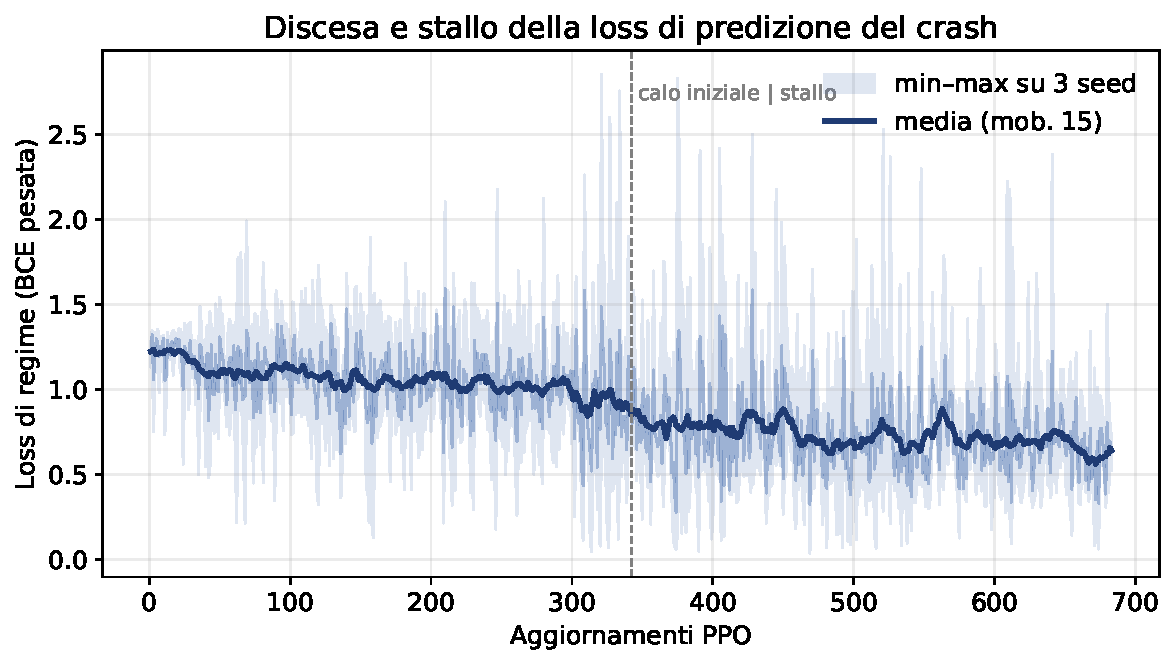
\includegraphics[width=0.8\linewidth]{regime_loss.pdf}
\caption{Loss BCE di predizione del crash durante l'addestramento (media su 3
seed, banda min--max).}
\label{fig:regime-loss}
\end{figure}

\begin{table}[H]
\centering
\small
\caption{Esponente con loss di regime (BCE) vs esponente appreso dal solo reward
(Esp.~2) vs formula fissa $p=2$, universo large-cap (mediana su 3 seed).}
\label{tab:exp-regime}
\begin{tabular}{llcccc}
\toprule
Periodo & Strategia & cash & MDD & Calmar & Sharpe \\
\midrule
\multirow{3}{*}{2015--26}
 & formula $p{=}2$      & $0.34$ & $0.138$ & $1.35$ & $1.44$ \\
 & appreso (reward)     & $0.37$ & $0.122$ & $1.41$ & $1.42$ \\
 & appreso + BCE        & $0.31$ & $0.166$ & $1.20$ & $1.44$ \\
\midrule
\multirow{3}{*}{COVID}
 & formula $p{=}2$      & $0.71$ & $0.067$ & $4.13$ & $2.52$ \\
 & appreso (reward)     & $0.74$ & $0.059$ & $4.06$ & $2.50$ \\
 & appreso + BCE        & $0.63$ & $0.090$ & $3.49$ & $2.32$ \\
\midrule
\multirow{3}{*}{2022}
 & formula $p{=}2$      & $0.78$ & $0.128$ & $-0.95$ & $-1.60$ \\
 & appreso (reward)     & $0.81$ & $0.111$ & $-0.95$ & $-1.61$ \\
 & appreso + BCE        & $0.68$ & $0.155$ & $-0.95$ & $-1.50$ \\
\midrule
\multirow{3}{*}{2025}
 & formula $p{=}2$      & $0.27$ & $0.119$ & $1.16$ & $1.09$ \\
 & appreso (reward)     & $0.31$ & $0.111$ & $1.19$ & $1.10$ \\
 & appreso + BCE        & $0.27$ & $0.123$ & $1.09$ & $1.09$ \\
\bottomrule
\end{tabular}
\end{table}

In sintesi, fornire una supervisione esplicita all'esponente non cambia l'esito.
Il limite non è la modalità di addestramento
ma l'assenza nei dati di un segnale sfruttabile sulla direzione futura dei
rendimenti.



\subsubsection{Regolare l'esponente con una regola}
Dato le precedenti osservazioni abbiamo pensato di affidare la scelta su quale esponente usare a una regola fissa. 
Questo permette di adattare dinamicamente l'esponente in base alla volatilità di mercato. 
La regola implementata consiste nell'aumentare l’aggressività del taglio di esposizione, cioè l'esponente $p$, man mano che sale l’indice VIX.


Tuttavia, anche questa soluzione fallisce: la regola ibrida riesce a eguagliare o superare la miglior formula fissa in \textbf{al più uno scenario su cinque}, sia in termini di drawdown che di Sharpe ratio.

Ci sono tre ragioni principali per cui questa soluzione non funziona:
\begin{enumerate}
    \item \textbf{Il compromesso diluisce l'efficacia:} variare $p$ in modo progressivo crea un'esposizione intermedia che finisce per non essere ottimale in nessun contesto: taglia troppo poco nei crolli improvvisi e troppo presto nelle fasi di lenta correzione.
    \item \textbf{Il VIX è un segnale reattivo, non predittivo:} il VIX non anticipa le crisi, ma esplode quando il crollo è già iniziato. Quando la regola rileva un picco di volatilità e decide finalmente di alzare l'esponente a $p=2$, la perdita di capitale si è già avvenuta in gran parte.
    \item \textbf{Asimmetria informativa:} capire se una discesa dei mercati sia l'inizio di un ribasso prolungato (dove servirebbe $p=1$) o di uno shock istantaneo (dove servirebbe $p=2$) è possibile solo a posteriori, mai in tempo reale mentre il fenomeno sta avvenendo.
\end{enumerate}

Quindi, un sistema difensivo basato su un segnale che arriva tardi non può impedire il danno. 
È come chiudere la porta dopo che il ladro è entrato. 
Il meccanismo di difesa si attiva, ma ormai i danni sono fatti.

\begin{table}[H]
\centering
\small
\caption{Esperimento 3: regola morbida sul VIX ($p:1\!\to\!2$ via
sigmoide) contro $p=1$ e $p=2$ fissi, in inferenza dallo stesso checkpoint
($\sigma_{\mathrm{target}}=0.20$, mediana su 3 seed).}
\label{tab:exp3-regola}
\begin{tabular}{llccccccc}
\toprule
Periodo & Modalita' & cash & MDD & Calmar & Sharpe \\
\midrule
\multirow{3}{*}{2015--26}
 & $p=1$ fisso  & $0.171$ & $0.240$ & $1.02$ & $1.433$ \\
 & $p=2$ fisso  & $0.220$ & $0.184$ & $1.24$  & $1.463$ \\
 & regola VIX   & $0.183$ & $0.234$ & $1.01$ & $1.432$ \\
\midrule
\multirow{3}{*}{COVID}
 & $p=1$ fisso  & $0.451$ & $0.148$ & $3.41$ & $2.281$ \\
 & $p=2$ fisso  & $0.579$ & $0.097$ & $4.18$ & $2.477$ \\
 & regola VIX   & $0.510$ & $0.122$ & $3.62$ & $2.380$ \\
\midrule
\multirow{3}{*}{2022}
 & $p=1$ fisso  & $0.504$ & $0.240$ & $-0.95$ & $-1.421$ \\
 & $p=2$ fisso  & $0.688$ & $0.181$ & $-0.95$ & $-1.616$ \\
 & regola VIX   & $0.550$ & $0.235$ & $-0.95$ & $-1.534$ \\
\midrule
\multirow{3}{*}{2017}
 & $p=1$ fisso  & $0.005$ & $0.047$ & $9.67$ & $3.129$ \\
 & $p=2$ fisso  & $0.005$ & $0.047$ & $9.67$ & $3.132$ \\
 & regola VIX   & $0.005$ & $0.047$ & $9.67$ & $3.130$ \\
\midrule
\multirow{3}{*}{2025}
 & $p=1$ fisso  & $0.140$ & $0.171$ & $1.00$ & $1.048$ \\
 & $p=2$ fisso  & $0.173$ & $0.152$ & $0.95$ & $0.984$ \\
 & regola VIX   & $0.149$ & $0.165$ & $0.90$ & $0.982$ \\
\bottomrule
\end{tabular}
\end{table}


\subsection{Generalità: trasferimento su panieri diversi}

Per verificare se im modello abbia davvero la proprietà di generalità o se sia invece legato al paniere azionario su cui è stata addestrato, abbiamo fatto un test di trasferimento. Abbiamo applicato il modello direttamente a portafogli completamente nuovi, senza fargli vedere prima i dati e senza alcun ri-addestramento. 

Grazie alla sua architettura, il modello può gestire portafogli di qualsiasi dimensione e composizione. Lo abbiamo quindi messo alla prova su panieri dell'indice S\&P~500 molto eterogenei per volatilità, settore di appartenenza, numerosità ($N=5$ e $N=20$) e grado di correlazione interna.

Sul decennio 2015--2026 (Tab.~\ref{tab:baskets-longrun}), la capacità difensiva del modello dimostra di saper \textbf{generalizzare con successo}:
\begin{itemize}
    \item \textbf{Difesa attiva reale ($\mathrm{MDD\_gain} > 0$):} su tutti i sei panieri testati, il modello contiene la perdita massima meglio di una strategia passiva con identica liquidità media (cioé il MDD del modello è minore rispetto a una strategia che tiene una liquidità sempre pari alla media del modello dal 2015 al 2026). Si tratta quindi di una gestione dinamica che aggiunge valore concreto.
    \item \textbf{Reattività anticiclica ($\rho_{\text{cash,dd}} > 0$):} la correlazione positiva conferma che il modello alza la quota di contante ogni volta che il mercato comincia a crollare, a prescindere dal tipo di titoli in portafoglio.
    \item \textbf{Flessibilità sul numero di titoli:} il meccanismo funziona altrettanto bene sia con un paniere ristretto di sole 5 azioni (\emph{small5}) sia con uno più ampio di 20 (\emph{large20}). Inoltre, nel paniere ben diversificato e a bassa correlazione le prestazioni restano solide, eliminando la paura che mantenere fissi i titoli nel tempo penalizzasse la strategia.
\end{itemize}

Dai risultati emerge un vincolo strutturale: la difesa è simmetrica ($\text{down\_capt} \approx \text{up\_capt}$).
Il modello reagisce puramente alla volatilità complessiva del paniere a presciendere dal fatto che sia a rialzo o ribasso.
Non c'è quindi alcun tipo di previsione direzionale.

\begin{table}[H]
\centering
\caption{\textbf{Trasferimento sul periodo lungo (2015--2026).}
Modello finale ($p=2$, mediana su 3 seed) su panieri mai visti in addestramento.
$\mathrm{MDD\_gain}>0$: drawdown ridotto meglio di un cash fisso di pari entità media;
$\rho_{\text{cash,dd}}$: tendenza ad alzare il contante al peggiorare delle perdite.}
\label{tab:baskets-longrun}
\begin{tabular}{lcccccc}
\toprule
Paniere & MDD & Calmar & MDD\_gain & down/up capt & $\rho_{\text{cash,dd}}$ \\
\midrule
difensivi     & $0.150$ & $0.68$ & $+0.115$ & $0.92/0.92$ & $0.38$  \\
diversificato & $0.156$ & $0.84$ & $+0.165$ & $0.87/0.86$ & $0.69$  \\
large20       & $0.241$ & $0.85$ & $+0.059$ & $0.82/0.82$ & $0.65$  \\
small5        & $0.169$ & $0.81$ & $+0.165$ & $0.87/0.86$ & $0.71$ \\
ciclici       & $0.383$ & $0.16$ & $+0.109$ & $0.71/0.68$ & $0.65$ \\
growth        & $0.201$ & $0.95$ & $+0.150$ & $0.52/0.52$ & $0.59$ \\
\bottomrule
\end{tabular}
\end{table}

Il riscontro più significativo si vede dallo stress test nei regimi critici (Tab.~\ref{tab:baskets-stress}): insieme alla capacità difensiva, si trasferisce in modo identico anche il limite dell'approccio. 
\begin{itemize}
    \item \textbf{Nei crolli violenti e rapidi (Crash COVID 2020):} la volatilità esplode immediatamente facendo scattare subito i tagli di esposizione. Il modello ottiene una vittoria netta su ogni paniere ($\mathrm{MDD\_gain} > 0$ ovunque).
    \item \textbf{Nei mercati ribassisti lenti e logoranti (Bear market 2022):} il modello fallisce su tutti i panieri ($\mathrm{MDD\_gain} \le 0$). In questo scenario i prezzi scendono con costanza ma senza picchi clamorosi di volatilità. 
    Il modello quindi non riceve quei segnali che gli indicano quando ritirarsi dal mercato in maniera aggressiva. 
    Per questo tiene sempre la liquidità abbastanza alta ma non ha nessun timing utile da sfruttare finendo per far peggio di un null a cash costante.

\end{itemize}

Questo schema è esattamente lo stesso osservato sui dati di addestramento. 
Il fatto che compaia anche su panieri del tutto nuovi ne dimostra la natura universale: non è un'anomalia di un singolo set di azioni, ma una proprietà strutturale del volatility targeting.

\begin{table}[H]
\centering
\caption{Difesa nei regimi di stress, zero-shot (modello finale $p=2$, mediana su
3 seed).}
\label{tab:baskets-stress}
\begin{tabular}{lcc}
\toprule
Paniere & MDD\_gain (COVID) & MDD\_gain (2022) \\
\midrule
difensivi     & $+0.096$ & $-0.003$ \\
diversificato & $+0.056$ & $-0.011$ \\
growth        & $+0.041$ & $-0.027$ \\
large20       & $+0.065$ & $-0.034$ \\
small5        & $+0.057$ & $-0.007$ \\
ciclici       & $+0.002$ & $-0.013$ \\
\bottomrule
\end{tabular}
\end{table}

\begin{figure}[H]
\centering
\begin{subfigure}{0.48\textwidth}\centering
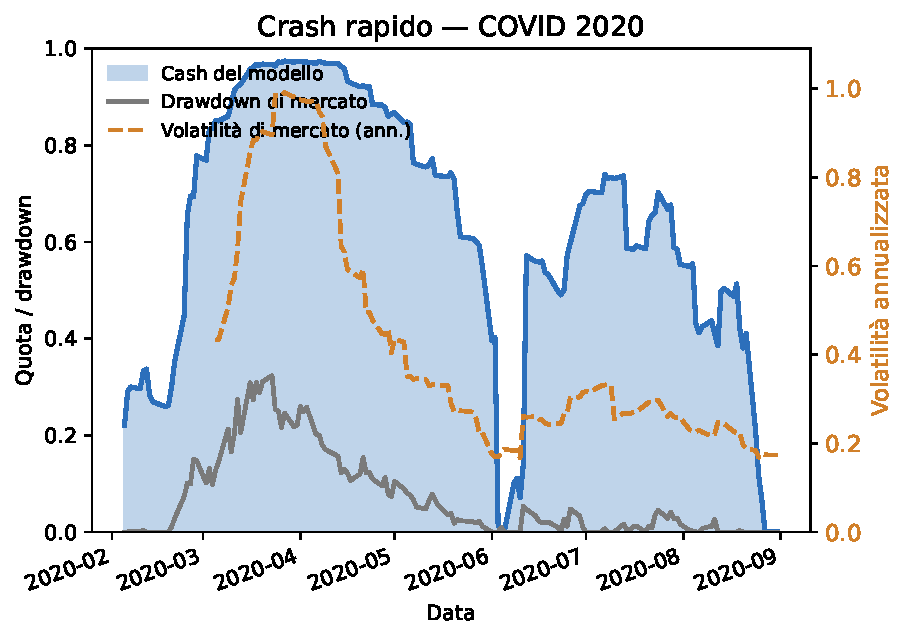
\includegraphics[width=\textwidth]{alloc_covid.pdf}
\caption{Crash rapido (COVID 2020)}
\label{fig:alloc-covid}
\end{subfigure}
\hfill
\begin{subfigure}{0.48\textwidth}\centering
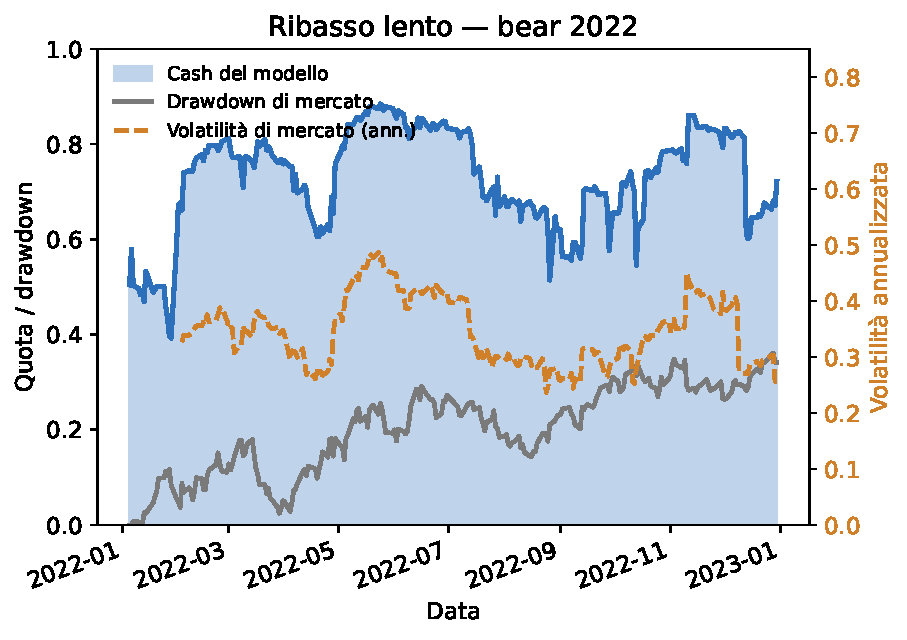
\includegraphics[width=\textwidth]{alloc_2022.pdf}
\caption{Ribasso lento (bear 2022)}
\label{fig:alloc-2022}
\end{subfigure}
\caption{Allocazione nel tempo: quota di liquidità del modello sovrapposta al drawdown/volatilità di mercato. Nel crash rapido (COVID) il cash sale in tempo; nel bear lento (2022) la volatilità resta bassa e la difesa arriva tardi.}
\label{fig:allocation-time}
\end{figure}


\subsection{Filo conduttore}
Ogni leva analizzata: $m_\theta$ calcolato, esponente stimato, regola in regime, non fornisce nulla che non si possa ottenere già scegliendo i parametri strutturali fissi ($\sigma_{\mathrm{target}}$ e esponente).
Il valore è completamente nella struttura, non nell'adattamento. 
La dipendenza dal regime è una caratteristica del mercato e non può essere utilizzata in tempo reale perché il regime è noto solo a posteriori. 
Il modello e la sua difesa si adattano a diversi universi, compresa la debolezza strutturale nei mercati lenti.




